%%%%%%%%%%%%%%%%%%%%%%%%%%%%%%%%%%%%%%%%%
% Structured General Purpose Assignment
% LaTeX Template
%
% This template has been downloaded from:
% http://www.latextemplates.com
%
% Original author:
% Ted Pavlic (http://www.tedpavlic.com)
%
% Note:
% The \lipsum[#] commands throughout this template generate dummy text
% to fill the template out. These commands should all be removed when 
% writing assignment content.
%
%%%%%%%%%%%%%%%%%%%%%%%%%%%%%%%%%%%%%%%%%

%----------------------------------------------------------------------------------------
%	PACKAGES AND OTHER DOCUMENT CONFIGURATIONS
%----------------------------------------------------------------------------------------

\documentclass{article}

\usepackage{fancyhdr} % Required for custom headers
\usepackage{lastpage} % Required to determine the last page for the footer
\usepackage{extramarks} % Required for headers and footers
\usepackage{graphicx} % Required to insert images
\usepackage{lipsum} % Used for inserting dummy 'Lorem ipsum' text into the template
\usepackage{listings}
\usepackage{color}
\usepackage{amsmath}
\usepackage{hyperref}
\usepackage{listings}

\lstset{frame=tb,
  language=matlab,
  aboveskip=3mm,
  belowskip=3mm,
  showstringspaces=false,
  columns=flexible,
  basicstyle={\small\ttfamily},
  numbers=none,
  numberstyle=\tiny\color{gray},
  keywordstyle=\color{blue},
  commentstyle=\color{dkgreen},
  stringstyle=\color{mauve},
  breaklines=true,
  breakatwhitespace=true
  tabsize=3
}

\definecolor{dkgreen}{rgb}{0,0.6,0}
\definecolor{gray}{rgb}{0.5,0.5,0.5}
\definecolor{mauve}{rgb}{0.58,0,0.82}

\lstset{frame=tb,
  language=python,
  aboveskip=3mm,
  belowskip=3mm,
  showstringspaces=false,
  columns=flexible,
  basicstyle={\small\ttfamily},
  numbers=none,
  numberstyle=\tiny\color{gray},
  keywordstyle=\color{blue},
  commentstyle=\color{dkgreen},
  stringstyle=\color{mauve},
  breaklines=true,
  breakatwhitespace=true
  tabsize=3
}

% Margins
\topmargin=-0.45in
\evensidemargin=0in
\oddsidemargin=0in
\textwidth=6.5in
\textheight=9.0in
\headsep=0.25in 

\linespread{1.1} % Line spacing

% Set up the header and footer
\pagestyle{fancy}
\lhead{\hmwkAuthorName} % Top left header
\chead{\hmwkClass\ (\hmwkClassInstructor\ \hmwkClassTime): \hmwkTitle} % Top center header
\rhead{\firstxmark} % Top right header
\lfoot{\lastxmark} % Bottom left footer
\cfoot{} % Bottom center footer
\rfoot{Page\ \thepage\ of\ \pageref{LastPage}} % Bottom right footer
\renewcommand\headrulewidth{0.4pt} % Size of the header rule
\renewcommand\footrulewidth{0.4pt} % Size of the footer rule

\setlength\parindent{0pt} % Removes all indentation from paragraphs

%----------------------------------------------------------------------------------------
%	DOCUMENT STRUCTURE COMMANDS
%	Skip this unless you know what you're doing
%----------------------------------------------------------------------------------------

% Header and footer for when a page split occurs within a problem environment
\newcommand{\enterProblemHeader}[1]{
\nobreak\extramarks{#1}{#1 continued on next page\ldots}\nobreak
\nobreak\extramarks{#1 (continued)}{#1 continued on next page\ldots}\nobreak
}

% Header and footer for when a page split occurs between problem environments
\newcommand{\exitProblemHeader}[1]{
\nobreak\extramarks{#1 (continued)}{#1 continued on next page\ldots}\nobreak
\nobreak\extramarks{#1}{}\nobreak
}

\setcounter{secnumdepth}{0} % Removes default section numbers
\newcounter{homeworkProblemCounter} % Creates a counter to keep track of the number of problems

\newcommand{\homeworkProblemName}{}
\newenvironment{homeworkProblem}[1][Apply MLT to Model 3D Chromatin Structures]{ % Makes a new environment called homeworkProblem which takes 1 argument (custom name) but the default is "Problem #"
\stepcounter{homeworkProblemCounter} % Increase counter for number of problems
\renewcommand{\homeworkProblemName}{#1} % Assign \homeworkProblemName the name of the problem
\section{\homeworkProblemName} % Make a section in the document with the custom problem count
\enterProblemHeader{\homeworkProblemName} % Header and footer within the environment
}{
\exitProblemHeader{\homeworkProblemName} % Header and footer after the environment
}

\newcommand{\problemAnswer}[1]{ % Defines the problem answer command with the content as the only argument
\noindent\framebox[\columnwidth][c]{\begin{minipage}{0.98\columnwidth}#1\end{minipage}} % Makes the box around the problem answer and puts the content inside
}

\newcommand{\homeworkSectionName}{}
\newenvironment{homeworkSection}[1]{ % New environment for sections within homework problems, takes 1 argument - the name of the section
\renewcommand{\homeworkSectionName}{#1} % Assign \homeworkSectionName to the name of the section from the environment argument
\subsection{\homeworkSectionName} % Make a subsection with the custom name of the subsection
\enterProblemHeader{\homeworkProblemName\ [\homeworkSectionName]} % Header and footer within the environment
}{
\enterProblemHeader{\homeworkProblemName} % Header and footer after the environment
}
   
%----------------------------------------------------------------------------------------
%	NAME AND CLASS SECTION
%----------------------------------------------------------------------------------------

\newcommand{\hmwkTitle}{Progress} % Assignment title
\newcommand{\hmwkDueDate}{Monday,\ May 12,\ 2014} % Due date
\newcommand{\hmwkClass}{Computational Biology} % Course/class
\newcommand{\hmwkClassTime}{} % Class/lecture time
\newcommand{\hmwkClassInstructor}{Jianyang Zeng} % Teacher/lecturer
\newcommand{\hmwkAuthorName}{Tianyi Hao, Weiyi Chen} % Your name

%----------------------------------------------------------------------------------------
%	TITLE PAGE
%----------------------------------------------------------------------------------------

\title{
\vspace{2in}
\textmd{\textbf{\hmwkClass:\ \hmwkTitle}}\\
\normalsize\vspace{0.1in}\small{Due\ on\ \hmwkDueDate}\\
\vspace{0.1in}\large{\textit{\hmwkClassInstructor\ \hmwkClassTime}}
\vspace{3in}
}

\author{\textbf{\hmwkAuthorName}}
\date{} % Insert date here if you want it to appear below your name

%----------------------------------------------------------------------------------------

\begin{document}

\maketitle

%----------------------------------------------------------------------------------------
%	TABLE OF CONTENTS
%----------------------------------------------------------------------------------------

%\setcounter{tocdepth}{1} % Uncomment this line if you don't want subsections listed in the ToC

%\newpage
%\tableofcontents
\newpage

%----------------------------------------------------------------------------------------
%	PROBLEM 1
%----------------------------------------------------------------------------------------

% To have just one problem per page, simply put a \clearpage after each problem

\begin{homeworkProblem}
	\begin{homeworkSection}{Overview}
	Since Prof. Jianyang Zeng has told Lingyu Wei and Zhengyu Wang performed well though didn't achieve a good result in this project. So in former two weeks we discussed with them about their former jobs in this project. We hope to develop our project based on their failure, or more exactly, based on their former progress. Last week we have implemented matlab code for their model and tried to analyze why the results of data experiment is not satisfiable. \\
	Roughly speaking, we believe the reason is from model. They have assumed the dependence between interaction frequency and distance is inverse, or later they modified it with one more intersect parameter. This is still too easy compared to the sophisticated 3D chromatin structure. In our future jobs, we will add more parameters and use different models (not just linear models) to iterate these experiment. If the problem still exists, we may need to think of another reason. On the other hand, there is a thought in our discussion. We found that, not only in their project but also in all our homework, the ratio sequence alignment is fixed, however in real world, based on some reports we read in the reference, this is changeable, should also be set as a parameter as well. So this time, we will make the comparison of our generated structure and original structure is by zooming in or out through enumeration. \\
	We hope this will help minimize the difference. In this progress report, we will explain what the problem is, how it shows up and how we generated these improving steps.
	\end{homeworkSection}
	
	\begin{homeworkSection}{Review: Manifold learning techniques and LLE}
		Manifold Learning pursuits the goal to embed data that originally lies in a high dimensional space in a lower dimensional space, while preserving characteristic properties. This is possible because for any high dimensional data to be interesting, it must be intrinsically low dimensional. High-dimensional data, meaning data that requires more than two or three dimensions to represent, can be difficult to interpret. One approach to simplification is to assume that the data of interest lie on an embedded non-linear manifold within the higher-dimensional space. If the manifold is of low enough dimension, the data can be visualized in the low-dimensional space. \\
		We follow the work by Saul and Roweis [1][2]. And the following is the original Locally Linear Embedding algorithm proposed in [1]. The main idea is that if the sample data are dense enough on a low dimensional manifold, any of the points can be approximately expressed as an affine combination of its neighbors. We reserve the affine combinations and fit the data points in a smaller dimension. 
	\end{homeworkSection}
	\begin{homeworkSection}{Review: Pseudocode}
		\begin{itemize}
			\item Parameter: K(The number of neighbors per point)
			\item Parameter: $X_1, ..., X_N \in R^D$
			\item Return: $Y_1, ..., Y_N \in R^d$
			\item Compute the nearest K neighbors of each data point X, as $\Gamma(i)$
			\item Compute the weighs $W_{i,j}$ that best reconstruct each data point $X_i$ from its neighbors, minimizing the cost in $E(W) = \sum_i |X_i - \sum_{j \in \Gamma(i)} W_{ij}X_j|^2$ subjected to $\sum_{j \in \Gamma(i)} W_{ij} = 1$ for every $i$.
			\item Compute the vectors $Y_i$ best reconstructed by the weights $W_{ij}$, minimizing the quadratic form $\Phi(W) = \sum_i |Y_i - \sum_{j \in \Gamma(i)} W_{ij}Y_j |^2$ by its bottom nonzero eigenvectors.
		\end{itemize}
	\end{homeworkSection}
	
	\begin{homeworkSection}{How we structure our code}
		We modify the LLE Algorithm a bit to fit in interaction frequency data. We can make $d=3$ in order to get three-dimensional points as the output. We can select the neighbors by the interaction frequency data because we can assume that the bigger frequency two fragments interact, the nearer they are. The most important step is the modification of step 2 in LLE, i.e., calculating $W_{ij}$ out of the interaction frequency data. We want to firstly try a very natural way of setting $W_{ij}$: proportional to the interaction frequency $f_{ij}$ ($f_{ij}$ is the interaction frequency between fragment $i$ and fragment $j$), i.e. 
		$$ W_{ij} = \frac{f_{ij}}{\sum_{j \in \Gamma(i)}f_{ij}} $$
		where $j \in \Gamma(i)$, otherwise $W_{ij} = 0$. \\
		We implement the algorithm in the matlab language currently. This is because Lingyu Wei and Zhengyu Wang were using matlab before, we were hoping the repeat their former experiment using the same data and libraries. After our analysis for their problem, we may still come back to use our python language, as illustrated in research proposal. \\
		The main algorithm is in $lle\_chroma.m$. Function $lle\_chroma$ uses $freq$ (interaction frequency matrix, whose size is $N*N$) and $K$ (the number of nearest neighbors to be considered) as input, and returns the embedding coordinates. 
		\begin{lstlisting}
function Y = lle_chroma(freq,K)
N = length(freq);

% STEP1: FIND NEIGHBORS 
[~,index] = sort(freq,'descend');
neighborhood = index(1:K,:);

% STEP2: SOLVE FOR RECONSTRUCTION WEIGHTS
W = zeros(N,N);
for j = 1:N
    W(neighborhood(:,j),j) = freq(neighborhood(:,j),j); 
end
W = W ./ repmat(sum(W),N,1);

% STEP 3: COMPUTE EMBEDDING FROM EIGENVECTS OF COST MATRIX M=(I-W)'(I-W)
M = eye(N) - W;
M = M*M' + eye(N); % Non-singular requirement

% CALCULATION OF EMBEDDING
options.disp = 0; options.isreal = 1; options.issym = 1; 
d = 3;
[Y,~] = eigs(M,d+1,0,options);
Y = Y(:,1:d)'*sqrt(N); % bottom evec is [1,1,1,1...] with eval 1
end
		\end{lstlisting}
		$Lle\_eval.m$ gives the implementation of evaluation function ($lle\_eval$), as well as input (readPDB) and output (printPDB) manipulation.
		\begin{lstlisting}
function Y = lle_eval(origin, outputfile, freq, p, K) % for example, inputfile = 'PMA_HoxA_Interactions.txt' and outputfile = 'out.pdb' and K = 7
    %[freq,p] = random_structure();
    Y = lle_chroma(freq,K);
    printPDB(origin, p);
    printPDB(outputfile, Y);
end

function freq = readPDB(filename)
    input = importdata(filename);
    data = input.data;
    first = min(min(data(:,1:2)))-1;
    last = max(max(data(:,1:2)));
    N = last-first;
    freq = zeros(N);
    for i=1:length(data)
        freq(data(i,1)-first,data(i,2)-first) = data(i,3);
    end
    freq = freq + freq';
end

function printPDB(filename, Y)
    fid=fopen(filename,'w');
    fmt = 'ATOM   % 4d C    LIG A        % 8.3f% 8.3f% 8.3f  1.00 75.00    \n';
    fprintf(fid,fmt, [(1:length(Y)); Y]);
    fprintf(fid,'CONECT % 4d% 4d\n', [(1:length(Y)-1);(2:length(Y))]);
	fprintf(fid,'END');
end
		\end{lstlisting}
	\end{homeworkSection}
	\begin{homeworkSection}{Dataset}
		In our proposal, we planned to conduct experiment on the data in [6,7] as our first test data for the compare of performance. However, after discussing with Zhengyu Wang, we were told he used to ask Prof. Jianyang Zeng where we can download the data. However the answer is nowhere. We were suggested by Lingyu Wei and Zhengyu Wang to generate data randomly. \\
		In other words, the structure is generated through a random walk and whose interaction frequency is obtained through the reciprocal to the distance, plus a random Gaussian perturbation. The code is implemented in $random\_structure.m$.
		\begin{lstlisting}
function [c,p] = random_structure()
N = 75;
p = zeros(3, N);
for i = 2 : N
    p(:,i) = p(:,i-1) + normrnd(0, 2, [3,1]);
end
plot3(p(1,:),p(2,:),p(3,:),'b*-');
c = zeros(N,N);
M = 10;
sig = 10;
for i = 1 : N
    for j = 1 : N
        if (i~=j) 
            c(i,j) = M / norm(p(:,i)-p(:,j), 'fro');%+randn();
        end
    end
end
		\end{lstlisting}
	In the next section, we will give the 3D embedding outcome for real data appeared in [6, 7], as illustrated in our research proposal. Then we will give the outcome of a simple empirical study on simulated data generated by the above function.
	\end{homeworkSection}
	\begin{homeworkSection}{Experiment}
	Real data experiment:
	\begin{itemize}
		\item Figure 1. The aligned embedding outcome of chromatin data from [6,7] \\
		\centerline{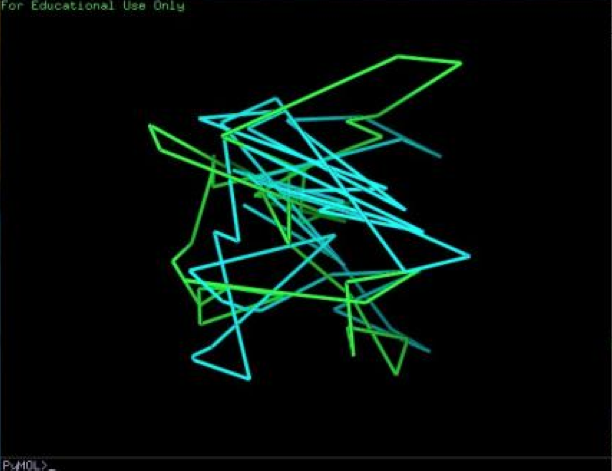
\includegraphics[scale=0.3]{Figure_1}}
		\item Figure 2. Undifferentiated State of Figure 1 \\
		\centerline{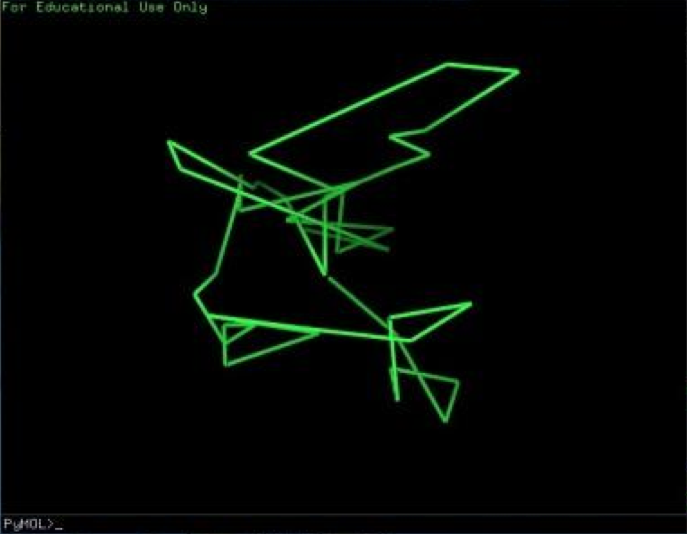
\includegraphics[scale=0.3]{Figure_2}}
		\item Figure 3. Differentiated State of Figure 1 \\
		\centerline{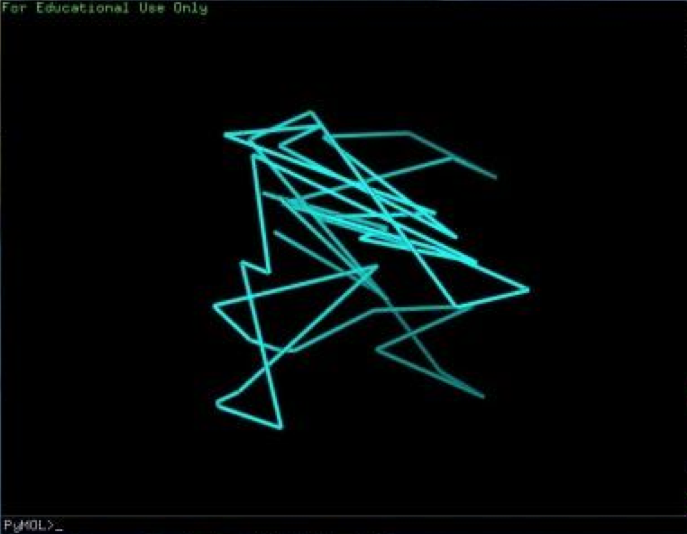
\includegraphics[scale=0.3]{Figure_3}}
	\end{itemize}
	Random data experiment:
	\begin{itemize}
		\item Original structure generated randomly \\
 		\centerline{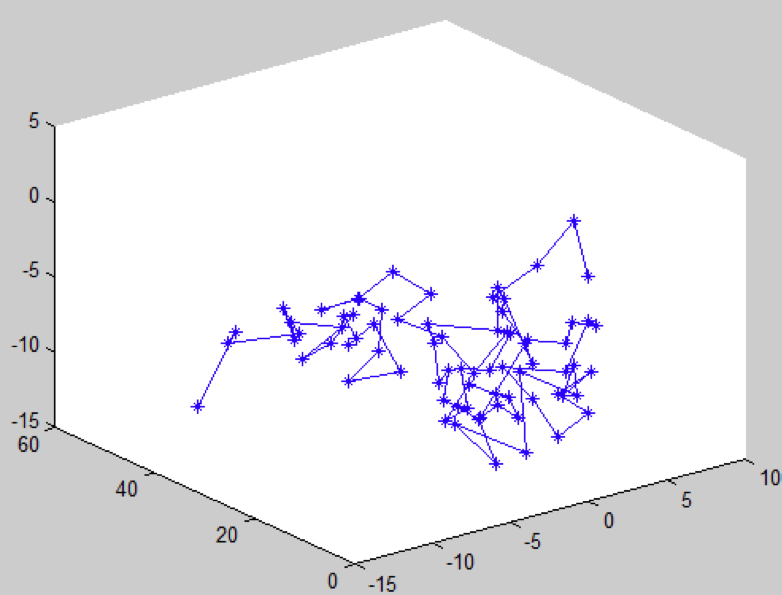
\includegraphics[scale=0.3]{Figure_4}} 
		\item Embedding with parameter $k = 3$ \\
		\centerline{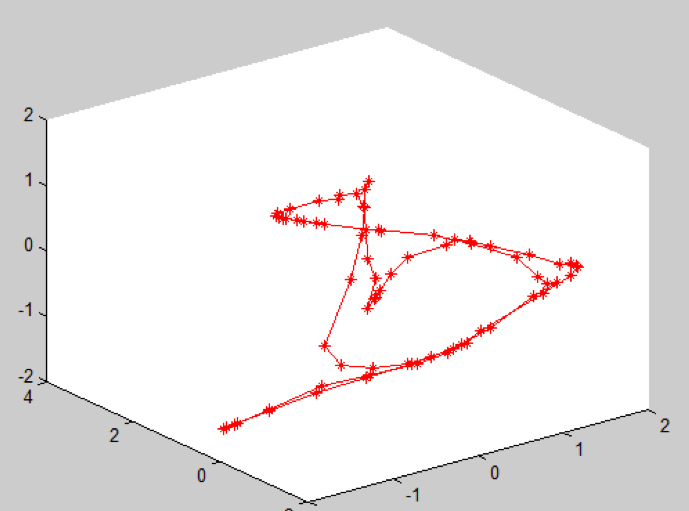
\includegraphics[scale=0.3]{Figure_5}} 
		\item Embedding with parameter $k = 7$ \\
		\centerline{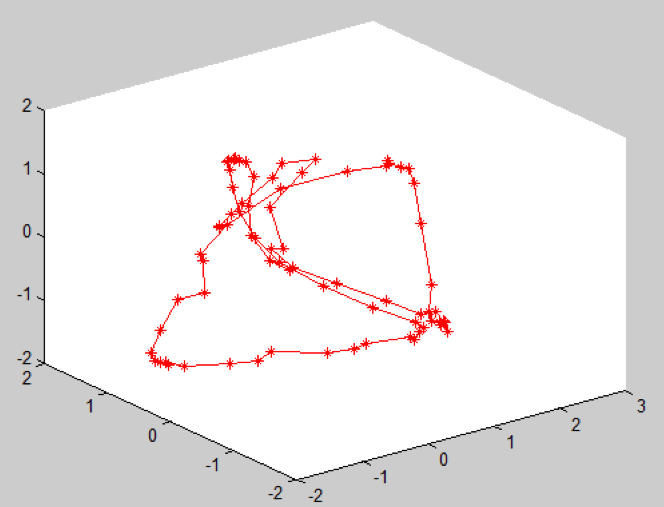
\includegraphics[scale=0.3]{Figure_6}} 
		\item Embedding with parameter $k = 15$ \\
		\centerline{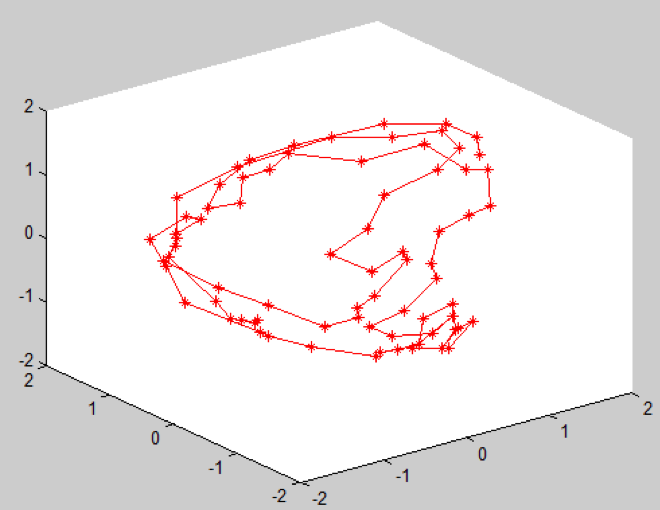
\includegraphics[scale=0.3]{Figure_7}} 
	\end{itemize}
	\end{homeworkSection}
	\begin{homeworkSection}{Reference}
		\begin{enumerate}
			\item L. Saul and S. Roweis, An Introduction to Locally Linear Embedding.
			\item S. Roweis and L. Saul, Nonlinear Dimensionality Reduction by Locally Linear Embedding. Science 290,pp.2323-2326 (2000) 
			\item \href{http://chromosome.sdsc.edu/mouse/hi-c/index.html}{\textcolor{blue}{Chromosome}}
			\item \href{http://www.cs.nyu.edu/~roweis/lle/}{\textcolor{blue}{CS NYU}}
			\item \href{http://en.wikipedia.org/wiki/Nonlinear_dimensionality_reduction}{\textcolor{blue}{Wiki Nonlinear dimensionality reduction}}
			\item Fraser J, Rousseau M, Shenker S, Ferraiuolo MA, Hayashizaki Y, Blanchette M, Dostie J.,Chromatin Conformation Signatures of Cellular Differentiation. Genome Biol. 2009;10(4):R37
			\item Rousseau M, Fraser J, Ferraiuolo MA, Dostie J, Blanchette M. Three-Dimensional Modeling of Chromatin Structure from Interaction Frequency Data Using Markov Chain Monte Carlo Sampling.BMC Bioinformatics. 2011.
		\end{enumerate}
	\end{homeworkSection}
\end{homeworkProblem}
\end{document}